\documentclass[10pt,twocolumn]{article}
% WS-076: rendered by make_paper.py from main.src.tex (do not edit main.tex). A generic 4-page two-column layout;
% swap the class for the target workshop's style file once the venue is chosen.
\usepackage[margin=0.75in]{geometry}
\usepackage{graphicx,amssymb,hyperref}
\usepackage[numbers]{natbib}
\title{Vision is the bottleneck: what transfers to the edge when a VLA runs on a Jetson Orin NX}
\author{Ravindu Somawansa\\Shisso Robotics}
\date{}
\begin{document}
\maketitle
\begin{abstract}
Training-free tricks promise faster or smoother execution of flow-matching vision-language-action policies, and they
are measured on desktop GPUs. On a Jetson Orin NX, a 450M SmolVLA spends 151.0 of 219.0 ms of
server time per action chunk in its vision encoder (69 \%, at 25 W). We measured seven of these tricks with one
checkpoint, the same 20 recorded episodes and bars committed before each run. A gradient-free prefix overwrite cuts the
boundary jump by 72--74 \% for 0.4 ms per chunk; projecting each chunk onto ten
movement primitives with a via-point at the seam removes 83--87 \% of the seam jerk at
+0.19$^\circ$ of error. Two Euler steps instead of ten save 41 ms (at MAXN) (17 \%). Exact real-time
chunking costs 1.9$\times$ a chunk; speculative selection (PACT) 1,200 ms per cycle, 37 control
ticks instead of 8; entropy-adaptive chunking 4,751 ms per decision. On the edge, overwrite the
prefix, smooth the seam, and leave the sampler alone.
\end{abstract}
\section{Introduction}
Robot-learning papers that speed up or smooth action chunking report their latencies on desktop and data-centre GPUs
(RTX 4090, A100, H100, RTX 5090), where a chunk costs tens of milliseconds and spare compute can hide an extra pass.
The robots people can buy run their policies on edge GPUs. We take one such setup --- an SO-101 arm, a Jetson Orin NX
16 GB, SmolVLA through a C++ engine (vla.cpp) --- and ask, for each trick, the question its paper does not: how much of
its benefit survives where the chunk is dominated by a cost the trick does not touch. Each answer is a pre-registered
gate: a bar committed before the number, an episode bootstrap for offline effects, medians of $\geq$ 50 calls for latency.

\section{Where the time goes}
A chunk at ten Euler steps costs 237.5 ms end to end on the Orin at full power (MAXN): 150.7 ms of vision,
14.9 ms of prefill and 5.3 ms per denoise step (Fig. 1; horizon $\times$ depth A2). At 25 W the server-side
split is 151.0 ms of vision in 219.0 ms (G-lat-2, bar commit \texttt{82fdc15}). Any trick that only
touches the denoising loop works on at most a quarter of the chunk.



\begin{figure}[t]\centering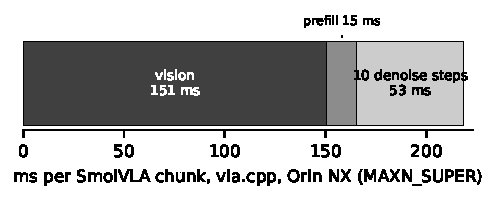
\includegraphics[width=\columnwidth]{fig/latency_split.pdf}\caption{Where a SmolVLA chunk's time goes on the Orin NX (vla.cpp, ten Euler steps).}\label{fig:split}\end{figure}

\section{Seven tricks, one checkpoint}
All offline effects use the same SmolVLA checkpoint and the same 20 recorded episodes (254 chunk boundaries per delay).

\textbf{Prefix overwrite vs exact real-time chunking (G13b).} Overwriting the new chunk's executed prefix with the
committed actions cuts the median boundary jump by 73 / 74 / 72 \% at delays of
8 / 12 / 20 steps (bar $\geq$ 50 \%); the exact guided inpainting of real-time chunking cuts it by 29 /
31 / 21 \% and costs 1962 ms per chunk in PyTorch against 1028 ms naive
(1.9$\times$). Ported to vla.cpp, the overwrite cuts 71 / 73 / 72 \% for
0.4 ms per chunk (Fig. 2).


\textbf{Movement-primitive projection and seam conditioning (smooth chunking, bar commit \texttt{6f58d7b}).} Projecting each
chunk onto ten Gaussian bases changes the error against the recorded continuation by -0.020$^\circ$ and removes
94 \% of the within-chunk jerk; conditioning on the last action sent removes 83 \% (25-step overlap)
and 87 \% (sync) of the seam jerk at +0.19$^\circ$. Both pass their bars.

\textbf{Two Euler steps (horizon $\times$ depth, bar commit \texttt{0a79846}).} Two steps contract the action cloud to
0.78 of its ten-step radius (CI 0.73--0.81; bar $\leq$ 0.70, paper 0.51): not proven. They save
41 ms per chunk (196.1 vs 237.5 ms, ratio 0.83).

\textbf{Speculative chunk selection (PACT-VLA, bar commit \texttt{0a79846}).} Choosing among four candidates with the
pre-commit frame picks chunks closer to the recorded teleop continuation (-0.27$^\circ$ against a random pick, CI
-0.44 to -0.09; one recorded continuation per frame, training-set episodes, open loop), but vla.cpp samples sequentially: the cycle costs 1,200 ms against 237.5 ms,
37 control ticks against 8, so "no added control-step delay" fails.

\textbf{Entropy-adaptive chunk length (AAC, bar commit \texttt{581a955}).} The chosen length sits at its floor in both phases
(median 2 steps in transport and 2 at the grasp), the median boundary-jump ratio with overwrite (the
step at the seam over the median step inside the chunk; lower is better) is 0.973 against 0.940 for fixed
chunks, and one decision with 20 samples costs 4,751 ms
against a 298 ms bar (Fig. 3).



\begin{figure}[t]\centering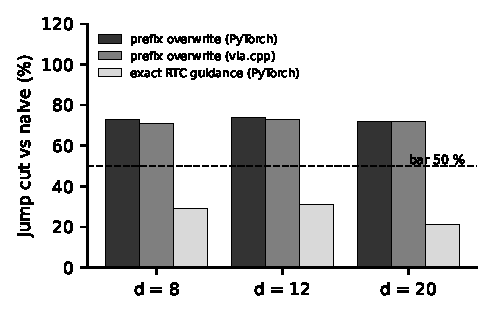
\includegraphics[width=\columnwidth]{fig/jump_cut.pdf}\caption{Median boundary-jump cut against naive asynchronous execution, 254 boundaries per delay.}\end{figure}
\begin{figure}[t]\centering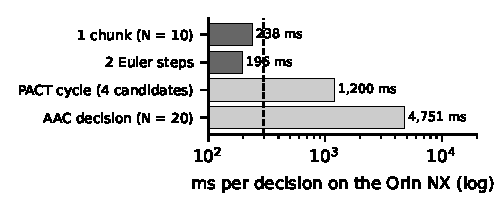
\includegraphics[width=\columnwidth]{fig/decision_cost.pdf}\caption{Cost per decision on the Orin NX; dashed: AAC's pre-registered bar.}\end{figure}

\section{The recipe, and what does not transfer}
Turn on the prefix overwrite and the primitive projection with seam conditioning: both act on the seam, which the
vision cost does not hide, and both cost under a millisecond. Keep ten Euler steps, by the protocol's rule (the two-step
contraction is not proven) rather than because the saving is unreal: it is real but small because vision dominates. Do not sample several chunks per decision on a sequential edge engine: every N-sample
method (exact guidance, PACT, AAC) pays N chunks in series. Arm results for the three transferring tricks are
\texttt{[to run]} (smooth chunking gate B, horizon $\times$ depth gate B, the overwrite in the robot client); they are the whole
addition of the 8-page version.

\section{Limitations}
One policy (SmolVLA, 450M); $\pi_0$-class models do not fit the Orin, which is itself part of the condition. vla.cpp is the
author's own port: it is measured against PyTorch on the same board (parity and determinism checks in the gate logs),
but an independent engine might move the sequential-sampling costs. Power mode is a confound: latency rows are at
MAXN\_SUPER unless stated, the G13b and G-lat-2 rows at 25 W. One task family (bowls), offline episodes for every effect
except latency; no arm success column yet.


\nocite{*}
\bibliographystyle{plainnat}
\bibliography{refs}
\end{document}
